
\subsection{Basic Blocked DGEMM}

I implemented the blocked \href{./../src/3-Optimize-Matrix-Matrix-Mult/dgemm-blocked.c}{DGEMM} has prescribed in the assignment and processed it on the cluster with different block sizes; the plots below \ref{fig:dgemm-performance} collect the timing traces.

\begin{figure}[h]
    \centering
    \begin{subfigure}[b]{0.48\textwidth}
        \centering
        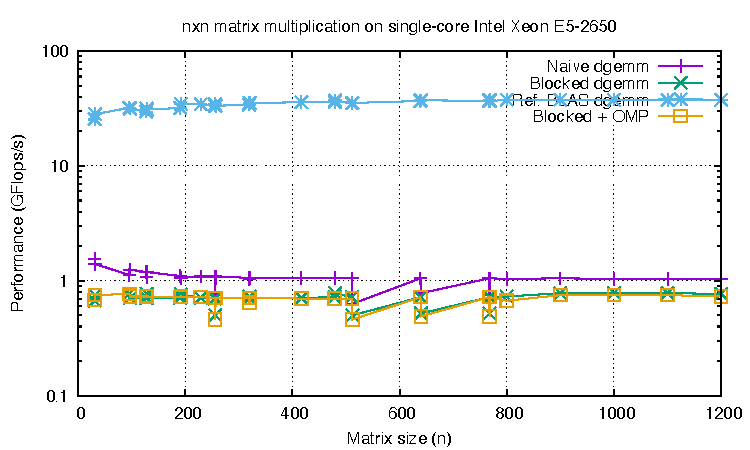
\includegraphics[width=\textwidth]{../src/3-Optimize-Matrix-Matrix-Mult/basic-dgemm-blocked/timing-02.pdf}
        \caption{Block size = 2}
        \label{fig:timing-02}
    \end{subfigure}
    \hfill
    \begin{subfigure}[b]{0.48\textwidth}
        \centering
        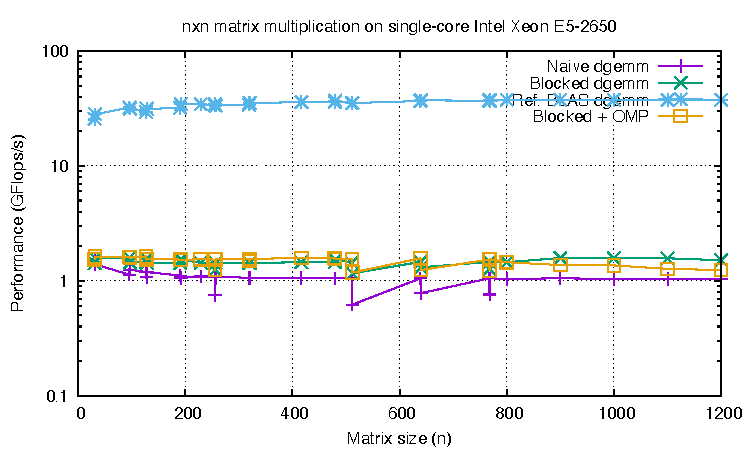
\includegraphics[width=\textwidth]{../src/3-Optimize-Matrix-Matrix-Mult/basic-dgemm-blocked/timing-04.pdf}
        \caption{Block size = 4}
        \label{fig:timing-04}
    \end{subfigure}
    
    \vspace{1em}
    
    \begin{subfigure}[b]{0.48\textwidth}
        \centering
        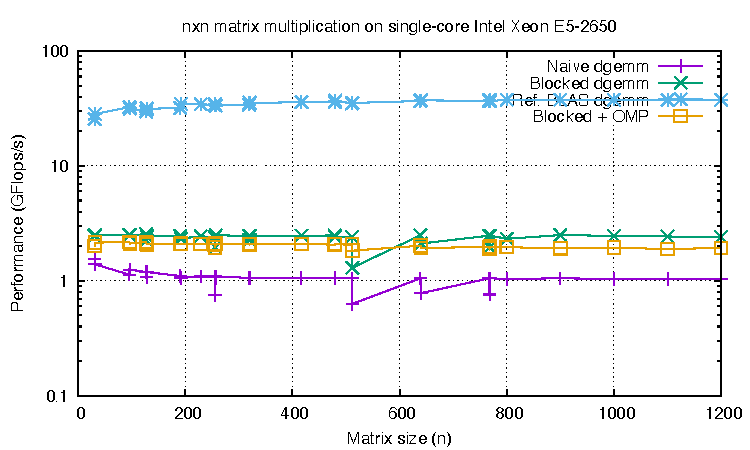
\includegraphics[width=\textwidth]{../src/3-Optimize-Matrix-Matrix-Mult/basic-dgemm-blocked/timing-08.pdf}
        \caption{Block size = 8}
        \label{fig:timing-08}
    \end{subfigure}
    \hfill
    \begin{subfigure}[b]{0.48\textwidth}
        \centering
        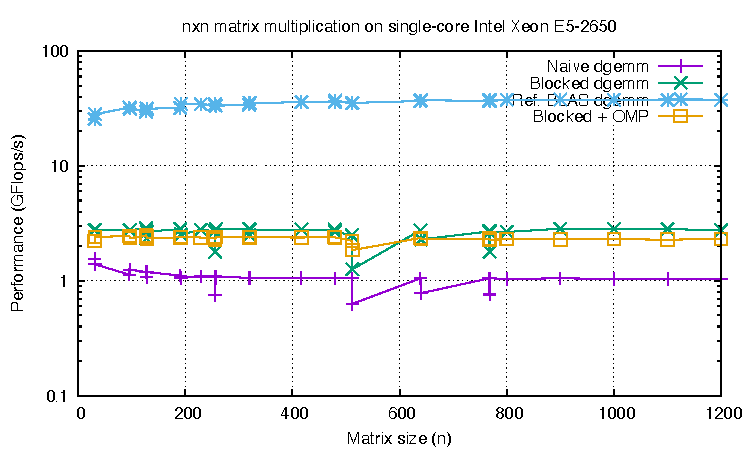
\includegraphics[width=\textwidth]{../src/3-Optimize-Matrix-Matrix-Mult/basic-dgemm-blocked/timing-16.pdf}
        \caption{Block size = 16}
        \label{fig:timing-16}
    \end{subfigure}
    
    \vspace{1em}
    
    \begin{subfigure}[b]{0.48\textwidth}
        \centering
        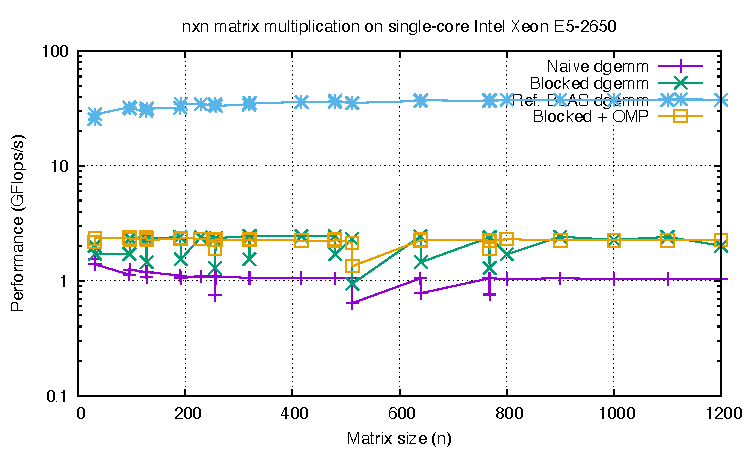
\includegraphics[width=\textwidth]{../src/3-Optimize-Matrix-Matrix-Mult/basic-dgemm-blocked/timing-32.pdf}
        \caption{Block size = 32}
        \label{fig:timing-32}
    \end{subfigure}
    \hfill
    \begin{subfigure}[b]{0.48\textwidth}
        \centering
        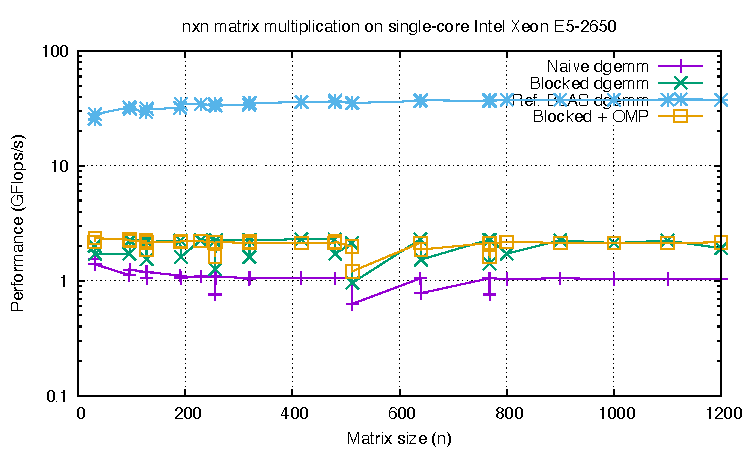
\includegraphics[width=\textwidth]{../src/3-Optimize-Matrix-Matrix-Mult/basic-dgemm-blocked/timing-64.pdf}
        \caption{Block size = 64}
        \label{fig:timing-64}
    \end{subfigure}
    
    \caption{Performance comparison of different DGEMM implementations with diffenet block sizes}
    \label{fig:dgemm-performance}
\end{figure}

I summarized each result from the \texttt{.out} file in the \href{./../src/3-Optimize-Matrix-Matrix-Mult/basic-dgemm-blocked}{basic-dgemm-blocked folder} and reported them in the Table~\ref{tab:performance-summary}. This includes the averages and the quick binary-search that made block size 16 the best result so far at 7.08\% of peak. Of course a more refinded search could still find a better configuration.

\begin{table}[h]
\centering
\caption{Average Percentage of Peak Performance}
\label{tab:performance-summary}
\begin{tabular}{|l|c|c|c|}
\hline
\textbf{Implementation} & \textbf{Block Size} & \textbf{Avg. \% Peak} & \textbf{Notes} \\
\hline
\hline
Naive DGEMM & -- & 2.88\% & Independent of block size \\
\hline
BLAS DGEMM & -- & 93.77\% & Reference implementation \\
\hline
\hline
\multirow{6}{*}{Blocked DGEMM} 
& 2  & 1.91\% & \\
\cline{2-4}
& 4  & 3.97\% & \\
\cline{2-4}
& 8  & 6.41\% & \\
\cline{2-4}
& 16 & 7.08\% & Best blocked performance \\
\cline{2-4}
& 32 & 5.54\% & \\
\cline{2-4}
& 64 & 5.37\% & \\
\hline
\end{tabular}
\end{table}


